\documentclass{article}

\usepackage[hidelinks]{hyperref}
\usepackage{graphicx}
\usepackage{titling}
\usepackage{float}
\usepackage[text={18cm,21cm},centering]{geometry}

\begin{document}

\begin{titlepage}
    \centering
    {\bfseries\LARGE Universidad de La Habana \par}
    \vspace{1cm}
    {\scshape\Large Facultad de Matemática y Computación \par}
    \vspace{3cm}
    {\scshape\Huge Primer Proyecto de Simulación (Inventario) \par}
    \vfill

    {\Large Anabel Benítez González C-411 \par}
    {\Large Raudel Alejandro Gómez Molina C-411 \par}
    \vfill
    {\href{https://github.com/anabel02/discrete-event-simulation}{Proyecto en github} \par}
\end{titlepage}

\section*{Introducción}

Este proyecto tiene como objetivo desarrollar una simulación de eventos discretos para entender mejor el problema orientado.
A través de este trabajo, buscamos aplicar los principios de la simulación de eventos discretos para modelar
y experimentar con estos fenómenos, y obtener resultados que nos ayuden a tomar decisiones informadas.


\subsection*{Objetivos y metas}
\begin{enumerate}
    \item Desarrollar un sistema que permita modelar el problema
    \item Utilizar el sistema para basándonos en sus resultados y en el análisis estádistico de estos, tomar decisiones.
\end{enumerate}

\subsection*{Sistema específico a simular}

\begin{itemize}
    \item Objetivos y metas
    \item El sistema específico a simular. ¿Qué es lo que se está simulando?
\end{itemize}

Para satisfacer las demandas, el tendero debe mantener una cantidad del producto a mano, y siempre que el inventario a
mano se vuelve bajo, se ordenan unidades adicionales al distribuidor. El tendero utiliza una política de pedido
llamada (s, S); es decir, siempre que el inventario a mano es menor que $s$ y no hay un pedido pendiente, entonces se
ordena una cantidad para llevarlo hasta S, donde $s<S$. Es decir, si el nivel de inventario actual es $x$ y no hay un
pedido pendiente, entonces si $x<s$ se ordena la cantidad $S-x$.
El costo de pedir y unidades del producto es una función especificada $c(y)$, y toma $L$ unidades de tiempo hasta que se
entrega el pedido, con el pago realizado a la entrega. Además, la tienda paga un costo de mantenimiento de inventario de
h por unidad de artículo por unidad de tiempo.
Supongamos además que siempre que un cliente demanda más del producto de lo que está disponible actualmente, entonces se
vende la cantidad a mano y el resto del pedido se pierde para la tienda.

El tendero está interesado en determinar el costo total esperado por unidad de tiempo para satisfacer la demanda del
producto:


\begin{itemize}

    \item Parámetros del sistema:
    \begin{itemize}
        \item  Tiempo máximo de la simulación ($t_{max}$).
        \item  Distribución del tiempo entre llegadas de los clientes ($T$).
        \item  Distribución de la demanda de los clientes para cada producto ($D$).
        \item  $s$, $S$, $L$, $h$, $c(y)$ para cada producto, $s_i$ es el nivel mínimo que debe alcanzar el producto $i$, $S_i$ es el nivel máximo que debe alcanzar el producto $i$, $L_i$ es el tiempo que toma en llegar el pedido del producto $i$,$h_i$ es el costo de mantenimiento de inventario por unidad de artículo por unidad de tiempo, $c_i(y)$ es el costo de pedir y unidades del producto $i$.
        \item Cantidad inicial de inventario ($I_0$).
        \item Cantidad inicial de dinero ($M_0$).
     \end{itemize}


    \item Variables de interés:
    \begin{itemize}
        \item Tiempo esperado en el que la ganancia supera una cantidad (esta cantidad pudiera ser la inversión inicial)
        \item Tiempo esperado en que el negocio quiebra (se queda sin dinero)
        \item Costo total esperado por unidad de tiempo para satisfacer la demanda del producto
        \item Valores de $s$ y $S$ que maximicen nuestra ganancia
    \end{itemize}
\end{itemize}


\section*{Detalles de la implementación}

En el directorio source se encuentran los archivos que contienen el código fuente de la simulación. El archivo \textbf{main.py}
es el punto de entrada de la simulación.
El módulo \textbf{simulation} contiene una abstractación de la simulación, y el módulo \textbf{inventory} contiene la implementación
para nuestro problema específico.

\subsection*{Simulation}

Contiene una implementación general de la simulación de eventos discretos.\\

En \textbf{core.py} encontramos:

\begin{itemize}
    \item La clase \textbf{Event} que representa un evento en la simulación. Cada evento tiene un tiempo asociado y una función \textbf{action} que ejecuta el evento.
    \item La clase \textbf{State} que representa el estado de la simulación.
    \item La clase \textbf{ActionByTime} que representa una acción que se ejecutará antes de cada evento programado.
\end{itemize}

En \textbf{simulator.py} encontramos:

\begin{itemize}
    \item La función \textbf{simulation} que recibe como parámetros una cola con prioridad de eventos, una instancia de \textbf{ActionByTime},
  el estado
  inicial de la simulación, el tiempo máximo de la simulación y una función que determina si la simulación debe
  detenerse. La función ejecuta la simulación de la siguiente manera:
  Mientras haya eventos en la cola, se extrae el primer evento, si el tiempo del evento es menor o igual al tiempo
  máximo de la simulación, se ejecuta la acción de \textbf{ActionByTime}, luego se revisa si se cumple el caso de parada, en caso
  negativo se ejecuta el evento y se actualiza el estado de la simulación, y se vuelve a revisar si se cumple el caso de
  parada con este nuevo estado.
    \item La simulación se detiene por alguno de los siguientes 3 motivos:
    \begin{itemize}
        \item Se alcanza el tiempo máximo de la simulación.
        \item Se cumple el caso de parada definido en \textbf{stop\_case}.
        \item Se terminan los eventos programados.
    \end{itemize}
\end{itemize}

\subsection*{Inventory}

Contiene la implementación específica de \textbf{simulation} para el problema de inventario.\\

En \textbf{inventory.py} se definen:

\begin{itemize}
    \item La clase \textbf{InventoryState} que representa el estado del inventario.
    \item La clase \textbf{RefillEvent} que representa el evento de reabastecimiento del inventario.
    \item La clase \textbf{SaleEvent} que representa el evento de venta de un producto.
    \item La clase \textbf{InventoryConfig} que representa la configuración del inventario.
    \item La clase \textbf{ActionByTimeInventory} que representa la característica de nuestro problema de pagar el costo de
  mantenimiento de inventario por unidad de artículo por unidad de tiempo.
\end{itemize}

En \textbf{inventory\_simulation.py} se define:

\begin{itemize}
    \item La función \textbf{inventory\_simulation} que recibe como parámetros el tiempo máximo de la simulación, la distribución del
  tiempo entre llegadas de los clientes, la lista con configuraciones del inventario, la distribución de la demanda de
  los clientes
  para cada producto, la cantidad inicial de cada producto en el inventario, la cantidad inicial de dinero y una función
  que determina si
  la simulación debe detenerse.
  La función primeramente verifica la consistencia de los parámetros (revisa que las listas que describen los productos
  tengan igual tamaño), luego inicializa el estado de la simulación, crea la cola con prioridad de eventos y ejecuta la
  simulación descrita en el módulo anterior.

    \item  ¿Cómo se crea la cola de eventos?
  Se inicializa una lista vacía.
  Por cada producto en la lista de configuraciones del inventario, se agregan eventos de venta hasta que el tiempo del
  evento sea mayor al tiempo máximo de la simulación.
  Se ordena la lista de eventos por tiempo y se devuelve.
\end{itemize}

\section*{Resultados y Experimentos}

Imaginemos que somos el tendero de una tienda que oferta un único producto y deseamos comparar distintos valores de s y S para maximizar nuestra ganancia media en una semana.

\vspace{\baselineskip}

¿Cómo podemos usar nuestro sistema para esto? Lo ejemplificamos en samples.ipynb.

\vspace{\baselineskip}

Nuestro modelo tiene esta forma:
\begin{itemize}
    \item Unidad de tiempo: hora
    \item  Tiempo máximo de la simulación $t_{max} = 24 \cdot 7$.
    \item  Distribución del tiempo entre llegadas de los clientes $T \sim Exp(\beta = 8)$.
    \item  Distribución de la demanda de los clientes para el producto $D \sim U(1,10)$.
    \item Unidades de tiempo que toma en llegar el pedido del producto $L = 3$
    \item Costo de mantenimiento de inventario por unidad de artículo por unidad de tiempo $h=1/100$
    \item Costo de pedir y unidades del producto $c(y) = y \cdot 50$
    \item Precio al que se vende una unidad de producto $p = 100$
    \item Cantidad inicial de inventario $I_0 = S$. Inicialicemos el almacén lleno.
    \item Cantidad inicial de dinero $M_0 = 0$.
\end{itemize}

Probemos fijando s y variando S:
\begin{itemize}
    \item Nivel mínimo que debe alcanzar el producto $s = 25$
    \item Nivel máximo que puede haber de producto en el almacén i:
    $S_1 = 110$ y $S_2 = 80$
\end{itemize}

¿Cómo comparamos nuestros sistemas?

\vspace{\baselineskip}

Realicemos 100 simulaciones en cada uno, quédandonos con el dinero con el que terminaró cada simulación, hallemos las medias para cada sistema y vamos a compararlas. A continuación los resultados:
\begin{enumerate}
    \item La media del sistema con {S=110} fue aproximadamente 4900 con una desviación estándar de 1102.
    \item La media del sistema con {S=80} fue aproximadamente 3592 con una desviación estandar de 1472.
\end{enumerate}

A continuación podemos visualizar la dispersión de los datos en cada sistema:

\begin{figure}[H]
    \centering
    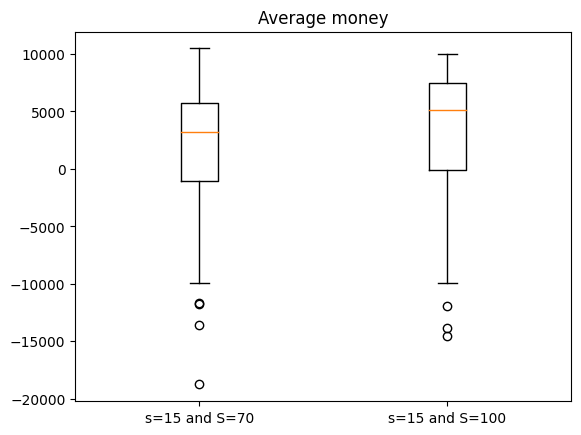
\includegraphics[width=0.7\linewidth]{./output.png}
    \label{fig:enter-label}
\end{figure}

Tanto en el gráfico como en los datos pudimos observar que se obtuvo mejores resultados con $S = 110$, o sea teniendo un almacén más grande.\\

Hagamos una prueba de hipotésis para comprobar si las diferencias son significativas o no: \\
    $H_o: \mu_1 = \mu_2 $\\
    $H_a: \mu_i \neq \mu_j$ \\
Cuando analizamos el intervalo de confianza con $\alpha=0.05$ de la diferencia entre ambos sistemas obtenemos  (-1647, -967) y como 0 no pertenece a este intervalo podemos rechazar la hipótesis nula y por tanto aceptar que nuestro sistema con $S=110$ tiene mejores resultados.

\section*{Modelo matemático}

\subsection*{Descripción}

Nuestro modelo matemático permite la simulación de un inventario de un establecimiento en los que los clientes llegan (definiendo intervalos de tiempo que distribuyen exponencial) y demandan cierto producto, esta demanda se rige por una variable aleatoria con distribución $D$. Si actualmente en el inventario no se dispone de la cantidad demandad por el cliente este no realiza la compra en caso contrario se abona el dinero correspondiente y la disponibilidad en el inventario disminulle. El abastecimiento del establecimiento se rige por una política $s$ - $S$, si el inventario se disminuye su volumen por debajo de $s$ se solicita un reabastecimiento de $S-k$ unidades donde $k$ es el volumen actual del inventario. Dicho reabastecimiento tiene un consto definido por una función $c(y)$ y demora $L$ unidades de tiempo. Además se paga un corto por almacenamiento definido por $h*k*it$ donde $it$ representa el intervalo de tiempo y $k$ el volumen del inventario durante ese período.

\subsection*{Variables implicadas en el modelo}

\begin{itemize}
    \item $t$ tiempo actual.
    \item $t_q$ tiempo asociado al evento que determina la llegada de un cliente.
    \item $t_y$ tiempo asociado al evento que determina un reabastecimiento.
    \item $k$ volumen del inventario.
    \item $x$ presupuesto actual.
    \item $y$ cantidad de volumen del reabastecimiento.
    \item $l$ tiempo que demora el reabastecimiento.
    \item $h$ costo por unidad de tiempo.
    \item $p$ precio de una unidad del producto.
\end{itemize}

\subsection*{Valores iniciales}

\begin{itemize}
    \item $t=0$.
    \item $t_q=q$ donde $q$ es una variable que distribuye exponencial.
    \item $t_y$ parámetro de la simulación.
    \item $k$ parámetro de la simulación.
    \item $x$ parámetro de la simulación.
    \item $y=0$.
    \item $l$ parámetro de la simulación.
    \item $h$ parámetro de la simulación.
    \item $p$ parámetro de la simulación.
\end{itemize}

\subsection*{Eventos}

\begin{enumerate}
    \item Llegada de un cliente: se actualiza $t=t_q$. Se genera una variable aleatoria $w$ con distribución $Q$, si $w<k$ no hacemos nada, en caso contrario $k=k-w$ y $x=x+p(w)$. Si $k<s$ se genera un evento reabastecimiento con $t_y=t+l$ y $y=S-k$. Dejar $t_q=t+q$ donde $q$ es una variable que distribuye exponencial (para analizar la próxima llegada).
    \item Llegada de un reabasteciemiento: se actualiza $t=t_y$. Se actualiza $k=k+y$ y $x=x-c(y)$.
    \item Calcular el costo de almacenamiento: se actualiza $x=x-h*it*k$.
\end{enumerate}

\subsection*{Supuestos y restricciones}

\begin{itemize}
    \item $c(y)$ costo del reabastecimiento de y unidades del producto.
    \item  Distribución del tiempo entre llegadas de los clientes $T \sim Exp(\beta = 8)$.
    \item  Distribución de la demanda de los clientes para el producto $D \sim U(1,10)$.
    \item  El evento de calcular el costo de almacenamiento ocurre antes de realizarse cada uno de los restantes eventos y luego de terminar la simulación.

\end{itemize}


\end{document}